\documentclass{dithesis}
\usepackage{mathspec}
\usepackage{xunicode}
\usepackage{enumitem}
\usepackage{ifthen}

% Math
\usepackage{amsfonts}

% Tikz
\usepackage{smartdiagram}
\usepackage{tikz}
\usetikzlibrary{arrows,mindmap,trees,fit,backgrounds,decorations.pathreplacing}

% Colors
\usepackage{xcolor}
\definecolor{num}{HTML}{FF7506}
\definecolor{myrd}{HTML}{B60005}
\definecolor{mybl}{HTML}{00706C}\definecolor{mygr}{HTML}{079500}
\definecolor{mybr}{HTML}{B85200}
\colorlet{myye}{yellow!30}

% Images
\usepackage{multicol}
\graphicspath{ {images/} }

% Code
%\usepackage{listings}
\usepackage{minted}

% URL
\usepackage{url}

\setallmainfonts[Mapping=tex-text]{Arial}
\setallsansfonts[Mapping=tex-text]{Arial}
\setallmonofonts[Mapping=tex-text]{Arial}

\renewcommand{\university}{National and Kapodistrian University of Athens}
\renewcommand{\school}{Faculty of Exact Sciences}
\renewcommand{\department}{Department of Informatics and Telecommunications}
\renewcommand{\thesisplace}{Athens}
\renewcommand{\thesisdate}{April 2016}
\renewcommand{\thesislabel}{Bachelor Thesis}
\renewcommand{\supervisorlabel}{Supervisors}
\renewcommand{\idlabel}{Α.Μ.}

\renewcommand{\contentsname}{Contents}
\renewcommand{\listfigurename}{List of Figures\vspace{5 mm}}
\renewcommand{\figurename}{Figure}
\renewcommand{\listtablename}{List of Tables\vspace{5 mm}}
\renewcommand{\tablename}{Table}
\renewcommand{\refname}{References}

\begin{document}

\newcommand{\op}[1]{
  	\node[draw,rounded corners,thick,fit={(0,.8)(5,1.2)}]{\newline #1};
}
\newcommand{\stream}[1]{
	\draw[->,very thick] (0,#1) -- (5,#1);
}
\newcommand{\dotstream}[2]{
	\draw[->,very thick] (0,#1) -- (#2,#1);
	\draw[dotted] (#2,#1) -- (5,#1);
}
\newcommand{\onnext}[4]{
	\draw (#1,#2) node [draw,circle,fill=#3] {\tiny #4};
}
\newcommand{\error}[2]{
	\draw[myrd, line width=1mm] (#1-0.3,#2-0.3) -- (#1+0.3,#2+0.3) (#1+0.3,#2-0.3) -- (#1-0.3,#2+0.3);
}
\newcommand{\complete}[2]{
	\draw[mygr, line width=1mm] (#1,#2-0.2) -- (#1,#2+0.2);
}

\newcommand\mat[2]{
	\node [rectangle,minimum size=5.5mm,inner sep=0pt,outer sep=0pt,thick,fill=mybr,opacity=.8] at (#1,#2) {};
}

\renewcommand\wr{
	\draw[red,thick,dashed,fit=(current bounding box.south west) (current bounding box.north east)];	 
	%\drawred,thick,dashed] (current bounding box.north west) -- (current bounding box.north east);
% \drawdecorate,decoration={brace,raise=2ex,mirror},very thick](current bounding box.north west) -- (current bounding box.south west);

}

% Minted settings
\newmintedfile[hs]{hs}{frame=lines,framesep=0.5cm}
\newmintedfile[jv]{java}{frame=lines,framesep=0.5cm}
\newmintedfile[scala]{scala}{frame=lines,framesep=0.5cm}
\usemintedstyle{bw}

\thesistitle{RHEA: A Reactive, Heterogeneous, Extensible and Abstract Framework for Dataflow Programming}
\thesisauthor{Orestis Melkonian}{1115201000128}
\supervisor{Panos Rondogiannis}{Professor EKPA}
\supervisor{Angelos Charalambidis}{Researcher NCSR}
\maketitle

\begin{thesisabstract}[Abstract]
Summary here

\thesiskeywords
{Subject Area}{Programming Languages}
{Keywords}
	{dataflow}
	{stream}
	{frp}
	{distributed systems}
	{model-driven architecture}
	{program synthesis}
	{declarative languages}
	{node placement}
\end{thesisabstract}

\begin{thesisdedication}
"τὰ όντα ιέναι τε πάντα καὶ μένειν ουδέν" \\
(all entities move and nothing remains still) \\
- Heraclitus
\end{thesisdedication}

\begin{thesisacknowledgments}[Acknowledgements]

I would like to thank Angelos Charalambidis for his immensely helpful supervision and guidance throughout the whole period of 6 months that I was present in NCSR. 

I would also like to thank Professor Panos Randogiannis for being a major influence in my current research interests through the undergraduate courses "Theory of Computation" and "Principles of Programming Languages", where I was introduced to a much more declarative way of programming and started appreciating mathematical sensibility in computing.

\end{thesisacknowledgments}

\tableofcontents
\listoffigures

\begin{thesisprologue}[Prologue]

This bachelor thesis is a continuation of my internship at the National Centre for Scientific Research "Demokritos", particularly in the Software and Knowledge Engineering Laboratory (SKEL). 

The main task I was assigned was the implementation of a framework for robot programming using a dataflow approach. During that internship, I came to realize that my work could be easily generalized to cover a much broader application area than just robot software. 

The name of the framework stems from the ancient Greek Titaness Rhea(\textit{Ρέα}), daughter of earth goddess Gaia(\textit{Γαία}) and sky god Uranus(\textit{Ουρανός}) and etymologically derives from the verb \textit{ρέω}(to flow).

\end{thesisprologue}


\thesissection{Introduction}

\thesissubsection{Main concept}

My main contribution is the design and implementation of a framework for dataflow programming to be deployed anywhere, ranging from low-performance robots and sensors to clusters of computer and even the Cloud. 

The main idea is to provide the programmer with a different execution model, the dataflow model, which allows for a more abstract way of thinking and has the advantage of exposing opportunities for parallelism (amongst CPU cores) and distribution (amongst computational machines) that the "intelligent" underlying system can automatically realize. Therefore, the programmer will be able to gain good performance and utilization of the available computational resources, while at the same time reducing development time and cost and maintaining a much cleaner and easier-to-refactor software system.


\thesissubsection{Motivation}

\thesissubsubsection{Declarative languages}

Software is becoming increasingly more complex each year, as computing capabilities are strengthened and user needs become more and more demanding. Thus the need for higher abstraction becomes mandatory, as it provides a more structured, easier to debug and maintainable way of developing software. In other words, abstraction in computer science acts as a mean to overcome complexity. 

In programming languages, the level of the aforementioned abstraction is measured regarding the amount of low-level details a programmer has to specify. Therefore, languages can be divided in two categories: the imperative ones, which specify what needs to be done and how to do it, and the declarative ones, which only specify what needs to be done and rely on the underlying compiler/interpreter to produce the exact commands that will realize the desired behaviour. The most well-known declarative programming paradigms are functional and logic programming, each providing higher abstraction in different aspects. My approach was greatly influenced by the functional paradigm.

\thesissubsubsection{Data versus Computation}			

A common problem in heterogeneous systems is that different representations of the same entities/data-types coexist in the same software and, as a consequence, pure computational tasks are intermingled with data-converting tasks. This makes the code less readable and harder to maintain and understand. In the dataflow execution model, there is a clear separation of these two aspects as data (edges) are completely decoupled from computation (nodes). This motivation is strengthened even more, when cross-machine communication is included, and apart from converting data from one representation to another, serialization(i.e. convertion to bytes) is also mandatory.

\thesissubsubsection{Dataflows in Robotics}

In control theory, which is the main background theory used in robotics, most architectures and/or algorithms are represented as dataflow diagrams for the sake of clarity and intuition. Translating these diagrams into common "imperative" software is not an easy tasks and is usually the source of bugs. Thus, having a dataflow execution model will nullify the need for such a translation.

Moreover, robotics typically involve several different robotic systems, whose combination is even more challenging. If each individual system is represented as a dataflow graph, composing them together is as trivial as connecting inputs with outputs, which is not the case in a traditional architecture, which is not component-based.

\thesissubsubsection{Dataflows in Big Data}

Another reason for following a dataflow approach is the attention that it recently has drawn in the Big Data field. As data size is growing exponentially and distribution is not a luxury but a necessity, a more scalable and decentralized architecture was destined to be examined in more depth. As we will discuss in the \textit{Related Work} chapter, there are many recent frameworks that became popular for the scalability due to the fact that they rely on a dataflow approach.

\thesissubsection{Outline}

There are nine chapters which compose this thesis: \textit{Introduction, Background, Approach, Implementation, Applications, Related Work, Future Work, Conclusions}.

\textit{Background} introduces the reader to basic background knowledge, necessary for complete understanding.

\textit{Approach} presents the main characteristics of my approach.

\textit{Implementation} gives a more detailed specification of the framework.

\textit{Applications} present some use-cases, ranging from general mathematical problems to real-life robot scenarios.

\textit{Related Work} discusses relevant concepts and technologies, which influenced major decisions concerning the design and implementation of the framework.

\textit{Future Work} suggests some interesting topics for future research, whose embedding in the framework is meaningful.

\textit{Conclusions} sums up.

\thesissection{Background}

\thesissubsection{The dataflow computational model}
The increased interest in parallelism during the 70's gave rise to the dataflow execution model, which is an alternative to the classical "von-Neumann" model. In the dataflow model, everything is represented in a dataflow graph, where nodes are independent computational units  and edges are communication channels between these units. A node/unit is fired immediately when its required inputs are available and therefore no explicit control commands are needed for execution. Figure 1 shows a dataflow graph enumerating the set $\mathbb{N}$ of natural numbers.

\mydiag{nat}{Natural numbers}	

The main advantage of the dataflow model is its implicit parallelism, deriving from the fact that the computational units are totally independent and therefore can be executed in parallel. The communication can either be an in-memory data storage or even a TCP connection across the network. Its great flexibility and composability make it a good candidate for the underlying architecture of a framework with a high level of abstraction.

\thesissubsection{Functional reactive programming}
A relatively recent model of programming is Functional Reactive Programming (FRP), which provides a conceptual framework for implementing reactive(i.e. time-varying and responding to external stimuli) behaviour in \textit{hybrid systems} (i.e. containing both continuous and discrete components), such as robots, in functional programming languages. It first appeared as a composable library for graphic animations \cite{fran}, but quickly evolved into a generic paradigm \cite{survey_frp,real_frp,pushpull_frp}. Moreover, extensive research has investigated FRP as a framework for robotics \cite{arrows_robots,lambda_in_motion}. \\
Although appealing at first, FRP was not appropriate for systems  with real-time constraints, due to uncontrollable time- and space- leaks \cite{event_frp}. The solution was a generalization of monads called \textit{arrows} \cite{arrows}, which provided the necessary guarantees that the aforementioned common errors do not occur. Let's see the example of calculating a robot's x-coordinate. Here is the mathematical formula drawn from control theory:

$$ x = 1/2 \int (vr + vl) \cos\theta $$ 

Below is the FRP code corresponding to the formula above:

\hs{code/frp1.hs}

As the above may seem counter-intuitive and difficult to understand, a new notation was conceived, notably the \textit{arrow notation} \cite{arrows_notation}:

\hs{code/frp2.hs}

The main advantages of FRP are its close correspondence to mathematics, which make it an ideal framework for modelling real-time systems, and its concise representation of time-varying values via \textit{signals}. \\
For a more detailed view of the FRP idiom and all of its variants please see the cited literature.

\thesissubsection{Publish-Subscribe model}

\textit{Publish/Subscribe}(PubSub) is a communication paradigm that became popular due to the loose coupling of its components, suited for the most recent large-scale distributed applications.

There is no point-to-point communication and no synchronization. \textit{Publishers} advertise messages of a given type to a specific message class or \textit{topic} that is identified by a \textit{keyword}, whereas \textit{subscribers} listen on a specific \textit{topic} without any knowledge of who the publishers are. The component responsible for relaying the messages between machines and/or processes and finding the cheaper dissemination method is called \textit{message broker}. Figure 2 illustrates an abstract representation of the PubSub model.

\mydiag{pubsub}{PubSub typical layout}

\thesissubsection{ROS: Robot Operating System}

\textit{ROS} is an open-source middleware for robot software, which emphasizes large-scale integrative robotics research \cite{ROS}. It provides a \textit{thin} communication layer between heterogeneous computers, from robots to mainframes and tt has been widely adopted by the research community around the world, due to its flexibility and maximal support of reusability through packaging and composability. It provides a nice solution to the development complexity introduced by complex robot applications that consist of several modules and require different device drivers for each individual robot. 

It follows a peer-to-peer network topology, implemented using a topic-based PubSub messaging protocol and its architecture reflects many sound design principles. Another great property of \textit{ROS} is that it is language-agnostic, meaning that only a minimal specification language for message transaction has been defined, so contributors are free to implement small-size clients in different programming languages, with \textit{roscpp} and \textit{rospy} being the most widely used ones.

A typical development scenario is to write several \textit{nodes}, that subscribe to some topics and, after doing some computation, publish their results on other topics. The main architectural issue here is that subscribing is realized through asynchronous callback functions, so complicated schemes easily lead to unstructured code, which obviously lead to unreadable and hard-to-maintain code. My approach gives a solution to the aforementioned problem.
 
\thesissubsection{Internet of things}

The birth of the Internet gave rise to a concept called \textit{Internet of Things} (IoT), which is essentially the ability of many heterogeneous devices, ranging from low-cost sensors to vehicles with embedded electronics, to collect data and exchange it amongst themselves using the Internet. This gave rise to smart grids, smart homes and eventually smart cities. 

The development of such systems though, due to their heterogeneity, is rather complex and costly. Typical software architectures were not meant to be used in such environments and therefore new tools and concepts needed to be invented. 

Fortunately, the dataflow model seems to be rather fitting for these scenarios, as every node in the graph is completely independent, and consequently can be any "\textit{thing}". This useful property of the model makes it a good architectural choice for such applications. The only thing to consider is how these things will communicate in a standard way, so as to be able to add new types of \textit{things} and integrate it in an effortless way to an existing dataflow network of \textit{things}.

\thesissubsection{The Strategy design pattern}

In software engineering, and especially in object-oriented programming(OOP), a \textit{design pattern} is a general repeatable solution to a commonly occurring problem in software design \cite{design}.

One such solution, the \textit{Strategy} design pattern is used when a particular algorithm can be implemented by a variety of behaviours/classes \cite{design}. In such a case, a good idea is to isolate the algorithm in a separate \textit{interface} and allow the system to select the appropriate instantiating classes at runtime.

Figure 3 illustrates the basic UML diagram of the strategy design pattern.

\begin{figure}[h!] 
	\centering
	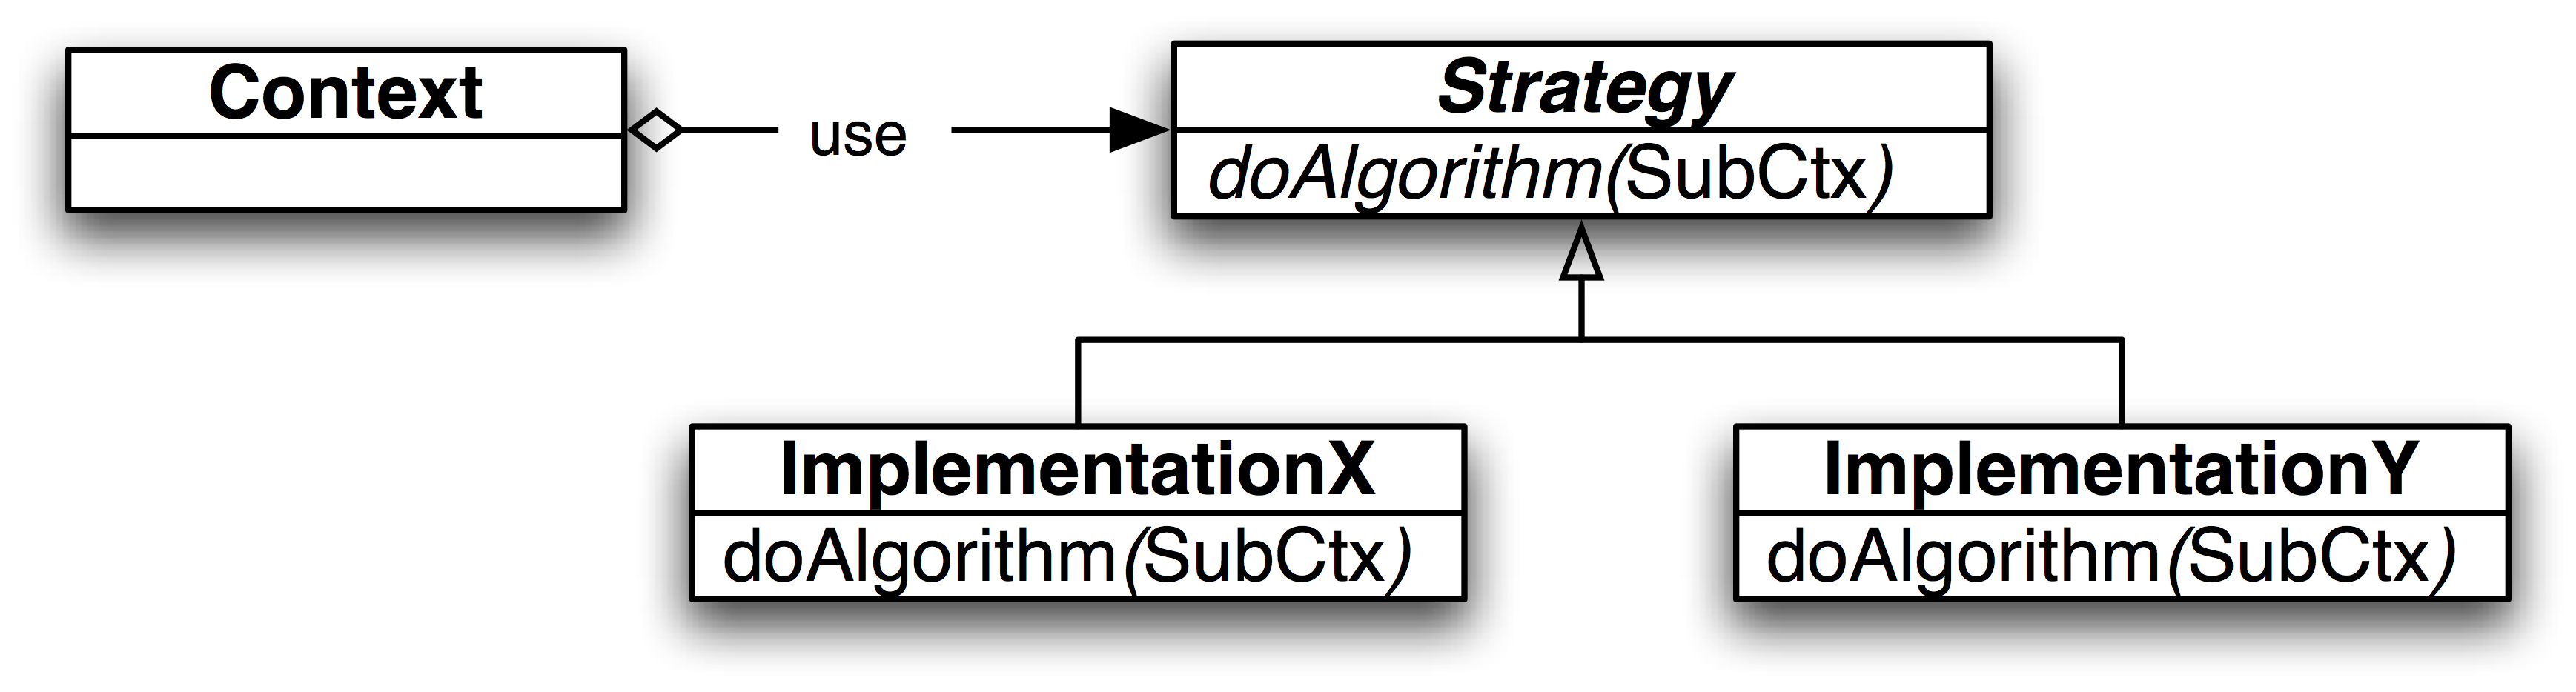
\includegraphics[scale=0.1]{strategy}
  	\caption{Strategy design pattern}
\end{figure}

\thesissection{Approach}
The design was heavily influenced by principles set out by the FRP and dataflow models. 

\thesissubsection{Reactive}

The system is \textit{reactive}, as close as possible to the definition of the Reactive Manifesto \cite{manifesto}. 

The system is \textit{responsive}, meaning it should be able to handle time-sensitive scenarios if at all possible. This is the cornerstone of usability and utility, but more than that, it enables quick error-detection and error-handling.

The system is \textit{resilient}, meaning it is able to recover robustly and gracefully after a failure, due to the fact that nodes in the dataflow graph are completely independent and recovery of each one can be done in textit{isolation}. Another thing to note here is that special error messages are built-in and make it very easy to propagate errors between \textit{components}, in case the error-handling part of a component is decoupled from the computational logic. This leads to much more robust architectures for large-scale systems, where fault-tolerance is mission-critical.

The system is \textit{elastic}, meaning it will adjust itself depending on the available resources and demanded workload. For instance, the granularity of the graph (i.e. number of nodes) is adjusted so as to match a heuristic-based value (e.g. total number of threads).

The system is \textit{message-driven}, meaning it relies solely on asynchronous message-passing for inter-component communication leading to loose coupling, isolation, location transparency and the error propagation mentioned above. Location transparency is critical to preserve the semantics whether on a single host or a machine cluster. 

\mydiag{manifesto}{Reactive properties}

\thesissubsection{Heterogeneous}

One of the major concerns while designing the framework was the ability to deploy it anywhere, from low-cost robots to mainframes. Obviously, such attribute would require a very flexible runtime environment. To satisfy this requirement, the strategy design pattern was used for evaluation, meaning that the core system only builds the internal representation of the dataflow graph and partitions it across the available computational resources. From there onwards, each partial graph can be evaluated by a different \textit{EvaluationStrategy} (see Implementation chapter), which could interpret it using the Java 8 Streams library or even compile into CUDA code for execution on a GPU.

Figure 5 illustrates a simple example of a robot application pipeline, where input to the dataflow graph is what the robot's camera senses, and after some image processing and some computation-heavy decision making, a command to an actuator of the robot is executed. Orange nodes are deployed on the robot's on-board computer, the green node is deployed on an off-board GPU and the red node is deployed on the lab's main cluster.

\mydiag{heterogen}{Heterogeneity pipeline}

\thesissubsection{Extensible}

While doing my internship at NCSR "Demokritos", I realized that the goal I was pursuing was impossible to reach closure in a 6-month period by a humble undergraduate student. Therefore, I decided that everything should be implemented in a way that will allow future contribution by me or other researchers/developers. 

With that concept in mind, I started generalizing and abstracting away everything I had done so far with the hope that the framework will raise attention later on. I can now say I am satisfied with the level of abstraction the core system has reached and I hope the stressful refactoring that the framework went through will blossom in the form of future contributions.

\thesissubsection{Abstract}

The framework is \textit{abstract} in terms of implementation details, as it is completely agnostic of any machine-specific or runtime-specific requirements. It is designed as a unifying conceptual base for further refined extensions and careful consideration was taken not to restrict in any aspect, architectural or not. The above was achieved by making many parts of the core system pluggable, which allows for easy refactoring on most of its internal functionality. Moreover, the internal graph representation does not include information on how a node is executed, but only what are its semantics.

\thesissection{Implementation}
This section examines the major characteristics of the framework's implementation.

\thesissubsection{Notifications}
Every value passed through the framework's \textit{streams} is wrapped inside a \textit{Notification} object, which discriminated stream values into three categories: \textit{onNext} (when the stream provides a regular value), \textit{onError} (when an error occurs) and \textit{onComplete} (when the stream completes its output).

\thesissubsection{The Reactive Streams Standard}
In order to make the framework easy to integrate with other stream and/or dataflow technologies, I decided that every input/output node (i.e. publisher/subscriber in the PubSub terminology or source/sink in the Dataflow terminology) should implement the interfaces that the Reactive Streams Standard (RSS) define. RSS is an initiative to provide a standard for asynchronous stream processing with non-blocking back pressure. This encompasses efforts aimed at runtime environments (JVM and JavaScript) as well as network protocols \cite{rss}.

A sink node (output) should implement the Subscriber interface \site{http://www.reactive-streams.org/reactive-streams-1.0.0-javadoc/org/reactivestreams/Subscriber.html}, which essentially defines three methods corresponding to reactions to a \textit{Notification}, one for each of the categories mentioned above. 

A source node (input) should implement the Publisher interface\site{http://www.reactive-streams.org/reactive-streams-1.0.0-javadoc/org/reactivestreams/Publisher.html}, which defines a single method \textit{subscribe(Subscriber s)}, where a Subscriber requests the Publisher to start emitting values. 

Many existing technologies provide these interfaces, or at least adapters from their internal representations, and therefore they are very easy to be integrated to the framework.

\newpage

\thesissubsection{Software structure}
The core system\site{https://github.com/rhea-flow/rhea-core} is organized in the following top-level packages:

\begin{tabularx}{\textwidth}{rX}
	\textit{org.rhea\_core.internal} 
	& all internal functionalities such as graphs, expressions and notifications \\
	\textit{org.rhea\_core.evaluation}
	& everything associated with the evaluation of the constructed dataflow graph \\
	\textit{org.rhea\_core.distribution}
	& everything associated with distributing the evaluation across the available computational resources \\
	\textit{org.rhea\_core.optimization}	
	& includes some built-in optimizers for adjusting the  granularity of the graph \\
	\textit{org.rhea\_core.io}
	& defines the interfaces that sources/sinks should implement \\
	\textit{org.rhea\_core.util}
	& helpful utilities needed throughout the project \\
\end{tabularx}

\thesissubsection{Internal representation}

For representing the internal structure of the dataflow graph, the \textit{JGrapht} open-source Java library was used, which provides many graph data structures and common graph-theory algorithms\site{http://jgrapht.org/}. The main class representing the internal dataflow graph is \textit{FlowGraph},  which is located in the \textit{org.rhea\_core.internal} package.

\thesissubsection{Stream variables}

The construction of the aforementioned internal graph is always implicit, through a rich set of stream operators. The only data type handled by the programmer is \textit{org.rhea\_core.Stream}, which contains the parametric type of its single output. Each \textit{Stream} object contains internally a \textit{FlowGraph}, which is only to be accessed and manipulated by the internal module, evaluation strategies and optimizers.

Figure 6 illustrates the dataflow graph(left) produced by the framework code(right) using the \textit{Stream} data type.

\usemintedstyle{autumn}
\codefig{simple}{\jv{code/simple.java}}{Simple stream example}

These variables can be used, preferably together with their parametric type, and reused in different parts of the graph. This is necessary, for instance, when you wish to split a node's output to different inputs. Figure 7 shows such an example.

\codefig{split}{\jv{code/split.java}}{Split example}

\thesissubsection{Stream operators}
This section displays the set of primitive operators, from which all the available stream operators are derived. Type information is not shown for the sake of readability, but all operations are type-safe.

In the marble diagrams on the right, circles represent \textit{onNext} notifications, green bars \textit{onComplete} and red x signals an \textit{onError}.

\newcommand{\lll}{0.4\linewidth}
\newcommand{\rrr}{0.4\linewidth}

\thesissubsubsection{Creation}
The following operators act as source nodes in the dataflow graph.
\begin{description}
\myitem{from}{(Iterable \textbf{i})}{none}{\textbf{i} as a stream}
\myitemm{fromSource}{(Source \textbf{s})}{none}{the values emitted by \textbf{s}}
\myitem{interval}{(TimeInterval \textbf{t})}{none}{the natural numbers emitted every \textbf{t}}
\myitem{empty}{~}{none}{an empty stream}
\myitem{never}{~}{none}{a stream that emits no notification}
\myitem{repeat}{(int \textbf{n})}{single}{repeats the values of the input stream \textbf{n} times, or infinitely if $\textbf{n} < 0$}
\myitemm{defer}{($\textbf{f}:() \to Stream$)}{none}{the stream generated by the given stream factory \textbf{f}}
\end{description}

\thesissubsubsection{Combining}
The following operators combine multiple streams to produce another one.
\begin{description}
\myitem{merge}{~}{many}{merges the input streams and completes as soon as any of them completes}
\myitem{concat}{~}{many}{concatenates the input streams in the given order}
\myitem{zip}{($\textbf{f}: A1...An \to B$)}{many}{zips the input streams with the given function \textbf{f}}
\end{description}

\thesissubsubsection{Filtering}
The following operators filter the values emitted by another stream.
\begin{description}
\myitem{filter}{($\textbf{f}: A \to Boolean$)}{single}{emits only values $i$ of the input stream, where $f(i) = true$}
\myitemm{filterMap}
{(\textbf{f}: A $\to$ B, \textbf{g}: B $\to$ Boolean)}{single}{emits only values $f(i)$ of the input stream the, where $(f \circ g)(i) = true$}
\myitem{distinct}{~}{single}{removes all duplicate values of the input stream}
\myitem{take}{(int \textbf{n})}{single}{extracts the first (last) \textbf{n} values of the input stream, if $\textbf{n} > 0 (< 0)$}
\myitem{skip}{(int \textbf{n})}{single}{skips the first (last) \textbf{n} values of the input stream, if $\textbf{n} > 0 (< 0)$}
\end{description}

\thesissubsubsection{Conditional}
The following operators behave depending on some conditions on their input stream
\begin{description}
\myitem{amb}{~}{many}{emits the values of one its input streams, whichever emits a value or terminates first}
\myitem{exists}{($\textbf{f}: A \to Boolean$)}{single}{returns True, if the input stream contains a value i, where $f(i) = true$ and False otherwise}
\myitemm{takeUntil}{(Stream \textbf{s})}{single}{extracts values of the input stream, until stream \textbf{s} emits a value}
\myitemm{skipUntil}{(Stream \textbf{s})}{single}{skips values of the input stream, until stream \textbf{s} emits a value}
\myitem{takeWhile}{($\textbf{f}: A \to Boolean$)}{single}{extracts values of the input stream until a value i is emitted, where $f(i) = false$}
\myitem{skipWhile}{($\textbf{f}: A \to Boolean$)}{single}{skips values of the input stream until a value i is emitted, where $f(i) = false$}
\end{description}

\thesissubsubsection{Transformational}
The following operators transform their input stream
\begin{description}
\myitem{map}{($\textbf{f}: A \to B$)}{single}{transforms the input stream by applying function \textbf{f} to every value emitted}
\myitem{scan}{(B seed, $\textbf{f}: B \times A \to B$)}{single}{transforms the input stream by sequentially applying function \textbf{f} to every value emitted  and emitting each result along the way}
\myitem{buffer}{(int \textbf{n})}{single}{packs together every \textbf{n} values of the input stream into a single List item}
\myitemm{buffer}{(TimeInterval \textbf{t})}{single}{packs together values of the input stream emitted every \textbf{t} into a single List item}
\end{description}

\thesissubsubsection{Feedback}
This operator enables cycles in the dataflow graph.
\begin{description}
\myitem{loop}{($\textbf{f}: Stream \to Stream$)}{single}{attaches a sub-graph to the input stream's output, whose result act as feedback to the attachment point}
\end{description}

\thesissubsubsection{Error-handling}
The following operators are a mean to handle errors.
\begin{description}

\myitemm{onErrorResume}{(Stream \textbf{s})}{single}{mirrors the input stream, but instead of emitting an \textit{onError} Notification when an error occurs, continues emitting values of the given stream \textbf{s}}
\myitem{onErrorReturn}{($\textbf{f}: Throwable \to A$)}{single}{mirrors the input stream, but instead of emitting an \textit{onError} Notification when an error e occurs, emits the value $f(e)$ followed by a \textit{onComplete} Notification}
\myitemm{retry}{(int \textbf{n})}{single}{mirrors the input stream, but instead of emitting an \textit{onError} Notification when an error occurs, resubscribes to it \textbf{n} times if $n > 0$, infinitely otherwise}
\end{description}

\thesissubsubsection{Backpressure}
The following operators specify how a node behaves when the requests are too intense to handle, computationally or memory-wise. \textit{Backpressure} is the mechanism that handles fast publishers that interact with slow subscribers.
\begin{description}
\myitemm{onBackpressureBuffer}{~}{single}{buffers values that cannot be handled by the subscriber to emit them later on}
\myitemm{onBackpressureDrop}{~}{single}{drops values that cannot be handled by the subscriber, instead of emitting them}
\myitemm{onBackpressureLatest}{~}{single}{drops values that cannot be handled by the subscriber and always buffers the last one, instead of emitting them}
\myitem{sample}{(TimeInterval \textbf{t})}{single}{emits only the most-recent emitted value from the input stream within intervals of \textbf{t}}
\myitemm{timeout}{(TimeInteval \textbf{t})}{single}{mirros the input stream, but emits \textit{onError} if there is no emission within time windows of \textbf{t}}
\end{description}

\thesissubsubsection{Utility}
The following operators provide some helpful utilities.
\begin{description}
\myitemm{doOnNext}{(Action \textbf{a})}{single}{execute Action \textbf{a} whenever onNext(Complete/Error) is called}
\myitemm{cache}{~}{single}{caches values emitted by the input stream for future subscribers}
\myitem{delay}{(TimeInterval \textbf{t})}{single}{emits the values of the input stream shifted forward in time by \textbf{t}}
\myitem{materialize}{~}{single}{wraps all values of input stream as Notifications}
\myitem{dematerialize}{~}{single}{reverses the effect of \textbf{materialize}}
\end{description}

All other operators can be produced by combining the above primitive ones \\
(e.g. $flatMap \equiv map \circ merge$).

\thesissubsection{Evaluation}

Every primitive operator corresponds to an expression implementing the \textit{Transformer} interface, defined in the \textit{org.rhea\_core.internal.expressions} package. 

A complete dataflow is defined by a \textit{Stream} variable and an object implementing the \textit{Output} interface, which can be either an \textit{Action}, a \textit{Sink} or a list of these. 

In order to evaluate a constructed dataflow graph the strategy design pattern is used, therefore a class implementing the \textit{EvaluationStrategy} interface, found in the \textit{org.rhea\_core.evaluation} package, needs to be provided. An \textit{EvaluationStrategy} just takes the \textit{Stream} variable and its corresponding \textit{Output} and executes it, however desired.

The strategies I have implemented so far follow:

\begin{description}[style=nextline]
\item[RxJavaEvaluationStrategy\site{https://github.com/rhea-flow/rx-eval}] 
Uses rxjava\site{https://github.com/ReactiveX/RxJava}, which is a famous and well-maintained library for asynchronous programming using the \textit{Observable} type, which is very close, semantically, to my \textit{Stream} variable.

\item[RosEvaluationStrategy\site{https://github.com/rhea-flow/ros-eval}] 
Integrates the \textit{ROS} middleware into the framework, by providing the \textit{RosTopic} class, which implements the \textit{AbstractTopic} interface defined in the \textit{org.rhea\_core.io} package. This strategy's job is to set up a \textit{ROS} client and configure every \textit{RosTopic} used within the dataflow that needs to be evaluated to use this client. After that, evaluation is propagated to a generic strategy (e.g. rxjava).

\item[MqttEvaluationStrategy\site{https://github.com/rhea-flow/mqtt-eval}] 
Integrates the MQTT middleware into the framework, in the same way \textit{ROS} is intergrated.
\end{description}

\thesissubsection{Distribution}

An evaluation strategy executes the requested dataflow graph in a single machine, without concern about distribution and resource utilization.

For distribution and cluster management, the strategy design pattern is used again, specifically the \textit{DistributionStrategy} interface, which is defined in the \textit{org.rhea\_core.internal.distribution} package. Its responsibility is to take the whole initial graph that we need to evaluate and, after adjusting its granularity (i.e. size) to fit the available resources (see \textit{Optimization} section), partition it across all computational resources, maybe using different evaluation strategies.

\thesissubsubsection{Hazelcast}

Due to the RSS being in its infant stage, no working implementation exists for superimposing a network protocol onto it (e.g. RSS over TCP). For this reason, I relied upon the open-source \textit{Hazelcast} library\site{http://hazelcast.org/} to discover and manage multiple machines and used its internal decentralized PubSub model to communicate intermediate results across the network. Figure 8 illustrates a dataflow graph on the left and the same graph partitioned over several machines on the right.

\twofig{partition1}{partition2}{Partitioning}

\thesissubsubsection{Machine configuration}

According to the distribution strategy being used, the available machines will require a certain initial configuration. For the \textit{Hazelcast} case, a little piece of setup code needs to be executed on every member of the cluster, which is together with the main \textit{Strategy} class. Moreover, helpful information can also be added at this step, such as number of CPU cores. It is the distribution strategy's responsibility to ensure that this information is properly distributed and handled.

Apart from this initial configuration, the distribution strategy needs to enable members to declare certain skills that they possess, which are required by specialized nodes. For instance, a source node emitting values from a \textit{ROS} topic must be executed on a machine having \textit{ROS} installed, in order to set up a \textit{ROS} client. In the \textit{Hazelcast} case, these skills are just \textit{strings} and are declared in the initialization code of each machine separately.

\thesissubsection{Optimization}

This section describes three stages of optimization the dataflow graph goes through before being evaluated. To aid extensibility  the strategy design pattern is again used, whose corresponding interface \textit{OptimizationStrategy} resides in the \textit{org.rhea\_core.optimization} package. Figure 9 illustrates the optimization stages.

\mydiag{optimization}{Optimization stages}

\thesissubsubsection{Proactive filtering}

The first optimization stage is a heuristic one, based on the fact that if a filter operation can be moved earlier (i.e. closer to source nodes) while preserving the original semantics, then there will be benefit concerning computational cost and across-machine communication overhead. The figures below show the corresponding graph transformations.

\optimization{maptake}{Take/skip/distinct before map}
\optimization{mapfilter}{Filter before map}
\optimization{concatdistinct}{Filter/distinct before concat/merge}

\thesissubsubsection{Granularity adjustment}

Different nodes of the dataflow graph will be executed on a separate thread/process. The fact that graphs can grow very big poses a problem when available computational resources are limited. For this reason, the second optimization stage tries to adjust the granularity of the dataflow graph to a desired value, which is the number of available threads amongst all machines. 

To achieve this, the optimizer applies some semantic-preserving transformation, as shown in the figures below (for simplicity, only a single example of each general case is demonstrated). 

\optimization{mergemap}{Merge maps}
\optimization{embedmap}{Embed map in creation}
\optimization{embedrepeat}{Embed repeat in creation}
\optimization{combmapfilter}{Combine map with filter}
\optimization{combfilterexists}{Combine filter with exists}
\optimization{combmapexists}{Combine map with exists}
\optimization{combmapzip}{Combine map with zip}
\optimization{combzipmap}{Combine zip with map}
\optimization{meaningless}{Meaningless nevers}

\thesissubsubsection{Node placement}

After the first two passes, we have an optimized dataflow graph with fine-tuned granularity. At this stage, nodes are mapped to tasks and are deployed across the available machines. 

If the desired granularity has not been reached yet, the \textit{DistributionStrategy} applies fusion to pairs of tasks until it reaches it, as shown in Figure 22.

\optimization{fusion}{Task fusion}

The final decision to be made is where each of these newly constructed tasks will be executed, although some of them need to necessarily be placed on specific machines with certain skills. 

Apart from these hard constraints, we need to minimize communication overhead. For this purpose, the strategy design pattern is again used, namely the \textit{NetworkProfileStrategy} that is defined in the \textit{org.rhea\_core.distribution} package. Its responsibility is to calculate a network distance between each pair of available machines, which is fed as input to the \textit{NodePlacement} optimizer. 

At this stage, we identify the aforementioned network distance as cost and apply brute-force to find the optimal placement of the (groups of) tasks that minimize that cost.

\thesissubsection{Serialization}

As communication between machines across a network is mandatory, data types emitted through the streams must be serialized on departure and de-serialized on arrival at each machine. For this reason, each \textit{DistributionStrategy} must be configured with a class implementing the \textit{Serializer} interface, define in the \textit{org.rhea\_core.serialization} package. The byte representation of the objects is parametric for maximum flexibility. 

A default \textit{Serializer} is provided with the core system, which can serialize every class implementing the \textit{Serializable} interface. In addition to that, the JsonIO library\site{https://github.com/jdereg/json-io} is used which allows serialization of many types of classes, but still does not cover every possible one. Figure 10 depicts the serialization process in more detail.

\mydiag{serialization}{Serialization process}

\thesissection{Applications}

\thesissubsection{Hamming numbers}
\thesissubsection{Camera surveilance}
\thesissubsection{Robot control panel}
\thesissubsection{Robot hospital guide}

\thesissection{Related Work}

This section discusses related work in the fields of \textit{Big Data}, \textit{Robotics} and \textit{IoT}.

\thesissubsection{Big Data}

The necessity for implicit parallelism and distribution of more and more applications, dealing with huge and/or complex data, has brought increasingly more attention to the dataflow programming model. Its easy to understand and maintain structure and declarative approach to programming, while not losing expressibility, has attracted many frameworks to utilize it.

\thesissubsubsection{GoogleDataflow}

Google recently released the \textit{GoogleDataflow }framework\site{https://cloud.google.com/dataflow/}, which is an evolution of \textit{FlumeJava}\cite{flumejava}, which in turn is a successor of the famous \textit{MapReduce }framework\cite{mapreduce}.

\textit{MapReduce} was a very simple model that allowed automatic concrrency/distribution on a cluster by allowing only a very minimal program structure. First, the user specifies a \textit{map} function that processes a key/value pair to generate a set of intermediate key/value pairs, and a \textit{reduce} function that merges all intermediate values associated with the same intermediate key. Although it was widely adopted at first, quickly many problems that could not be expressed with the above formalism were found and therefore a more expressive model was required.

This gave birth to \textit{FlumeJava}, which is a generalization of the \textit{MapReduce} framework that allows more expressive pipelines of more primitive operations like \textit{MapReduce}.

Although \textit{FlumeJava} was more attractive due to its expressibility, still the pipeline constructed could not formulate all problems that are needed in some big-data applications. For instance, the constructed dataflow could not contain cycles, which is an integral part of \textit{incremental computation}, used extensively nowadays for machine learning and data analysis.

And this is how \textit{GoogleDataflow} came to exist, offering a fully generic dataflow framework integrated with many other closely-related technologies from Google, like Cloud Storage\site{https://cloud.google.com/storage/}, Cloud PubSub\site{https://cloud.google.com/pubsub/}, Cloud Datastore\site{https://cloud.google.com/datastore/}, Cloud Bigtable\site{https://cloud.google.com/bigtable/} and BigQuery\site{https://cloud.google.com/bigquery/}. 

It is open-source, offers fully automatic resource management that auto-scales for optimal throughput and provides increased reliability and data consistency. Moreover, it provides a unified programming model through its API, while allowing data monitoring and demand-driven execution.

\thesissubsubsection{TensorFlow}

Another dataflow framework from Google is TensorFlow\site{https://www.tensorflow.org/}, which is an open-source polyglot library for machine learning and especially construction of neural networks.

The interesting fact is that, although it started out as a rigid neural network library, it quickly generalized to a dataflow construction library, much similar to my own project, which started out as a robotics library. 

Its main features are its portability to multiple computational architetures (e.g. CPU, GPU, etc...) and multiple language APIs (e.g. C++, Python), although its main advantage are its domain-specific operators for neural nets (i.e. common subgraphs, auto-differentiation).

Though the edges/streams connecting the nodes, only a single but flexible data type is allowed, namely the \textit{Tensor} type, which essentially is a multi-dimensional array that usually represents features or weights. Figure ? illustrates a neural network as a dataflow graph.

\myimage{tensorflow}{0.5}{TensorFlow graph}

\thesissubsubsection{Akka}

Definitely one the most mature frameworks for distribution targeting the JVM, \textit{Akka}\site{http://akka.io/} is a toolkit and runtime for highly concurrent, distributed and resilient message-driven applications. It is also one of the founders of the Reactive Streams\cite{rss} initiative.

Its approach follows the Actor model\cite{actor}, where one perceives abstract computational agents, called actors, that are distributed in space and communicate with point-to-point messages that are buffered in a queue. In reaction to a message, an actor can create more actors, make local decisions, send more messages and determine how to respond to the next message received.

Similar to the problem of \textit{ROS} that my framework solved, which is the inappropriate nature of callbacks for complex scenarios, \textit{Akka} developers also felt the same necessity for a more flexible and composable programming model, so they started the AkkaStreams library\site{http://doc.akka.io/docs/akka-stream-and-http-experimental/1.0-M2/scala.html} which provides a convenient API for stream processing and also dataflow graph construction with an interesting DSL. Figure ? demonstrates a dataflow graph on the left, generated by the DSL code on the right.

\usemintedstyle{friendly}
\codefig{akka}{\scala{code/akka.scala}}{Akka DSL}		

\thesissubsubsection{Spark}

A very well-known and well-adapted framework for scalable large-data processing is Apache's \textit{Spark}\site{http://spark.apache.org/}. It was developed to overcome the shortcomings of the \textit{MapReduce} framework mentioned above, providing a much more efficient and flexible runtime.

It follows the same general approach as \textit{RHEA}, meaning that it is completely generic and encourages domain-specific libraries to be built upon it. For instance, \textit{MLib}\site{http://spark.apache.org/mllib/} is a library for machine learning and \textit{GraphX}\site{http://spark.apache.org/graphx/} is a library for iterative graph algorithms, both sitting onto \textit{Spark}.

It offers a rich set of data-parallel operators ($\simeq 80$) that can be used interactively from Scala, Python, Java or R. The code below shows the classic word-counting example in Spark's Scala API.

\usemintedstyle{friendly}
\scala{code/spark.scala}

\thesissubsubsection{Naiad}

Offering the high throughput of batch processors, the low latency of stream processors and the ability to perform iterative and incremental computations at the same time is extremely challenging and none of the aforementioned frameworks manage to provide it. Applications that need all these features need to rely on multiple platforms, at the expense of efficiency, maintainability and simplicity.

Naiad\cite{naiad} combines all of these features in a unifying framework, that provides a generic low-level platform, that a wide variety of high-level programming models can be built upon, enabling such diverse tasks as treaming data analysis, iterative machine learning, and interactive graph mining.

Its main contribution is the definition of a new computational model, namely the \textit{Timely Dataflow} model, which is an extension to the dataflow model I introduced in the first chapter, by allowing a more efficient and lightweight coordination mechanism for capturing opportunities for parallelism. This is achieved by enriching the dataflow model with timestamps that represent logical points in the computation.

Figure ? shows a Naiad application that supports real-time queries on continually updated data.

\myimage{naiad}{0.7}{Naiad application}

\thesissubsubsection{dispel4py}

A less-known framework for Python is \textit{dispel4py}\site{https://github.com/dispel4py}. It provides the ability to describe abstract workflows for distributed data-intensive applications.

Similar to my \textit{EvaluationStrategy} concept, it allows different mappings to enactment systems, such as MPI\site{http://www.mcs.anl.gov/project/mpich-high-performance-portable-implementation-mpi} and Apache Storm\site{http://storm.apache.org/}.

Its main disadvantages are that only has a Python API and that it only allows low-level specification of the graph's nodes, through the definition of \textit{Processing Elements}. Therefore, it is impossible to compose larger graphs from simpler ones easily and the source code becomes chaotic and difficult to maintain.


\thesissubsection{Robotics}
\thesissubsubsection{Flowstone}
\thesissubsubsection{Yampa}
\thesissubsubsection{roshask}

\thesissubsection{Internet of Things}
\thesissubsubsection{NodeRed}
\thesissubsubsection{NoFlo}

\thesissection{Future Work}

\thesissubsection{More evaluation strategies}
\thesissubsection{Dynamic reconfiguration}
\thesissubsection{Advanced network profiling}
\thesissubsection{DSLs for framework extension}
\thesissubsection{Advanced fault-tolerance}
\thesissubsection{Integration with other technologies}
\thesissubsection{Visual language}
\thesissubsection{Stream reasoning}	

\thesissection{Conclusions}

\begin{thesisabbreviations}
A table of all abbrevations used throughout the thesis follows.

\begin{tabularx}{\textwidth}{|X|X|}
  \hline
  FRP & Functional Reactive Programming \\
  JVM & Java Virtual Machine \\
  NCSR & National Centre for Scientific Research \\
  ROS & Robot Operating System \\
  IoT & Internet of Things \\
  CPU & Central Processing Unit \\
  TCP & Transmission Control Protocol \\
  PubSub & Publish/Subscribe \\
  OOP & Object-oriented Programming \\
  UML & Unified Modelling Language \\
  GPU & Graphics Processing Unit \\
  DSL & Domain-specific Language \\
  RSS & Reactive Streams Standard \\
  API & Application Programming Interface \\
  MPI & Message Passsing Inteface \\
  \hline
\end{tabularx}

\end{thesisabbreviations}

\newpage
\bibliographystyle{ieeetr}
\bibliography{thesis}{}

\end{document}
